\cotefile{156-9}
\scanpage{90}
\mspage{86}
% archive sheet number: 89

et \unsure{on} trouve la $=$ interprétation pour le $2^{\mathrm e}$ \unsure{mbr|membre} de $\unsure{\alpha|\infty}$.

Soient maintenant $(E,\mid\circ\mid_E)$, $(E',\mid\circ\mid_{E'})$ deux \unsure{disjoncteurs}, et considérons deux correspondances
\[
\begin{aligned}
\alpha &: E \unsure{\text{---}|\longrightarrow} \unsure{\mathscr{P}|\mathcal{P}}(E') \quad,\quad \bar\alpha : \mathscr{P}(E)\unsure{\text{---}|\longrightarrow}\mathscr{P}(E')\\
\beta &: E'\unsure{\text{---}|\longrightarrow}\mathscr{P}(E) \quad,\quad \bar\beta : \mathscr{P}(E')\unsure{\text{---}|\longrightarrow}\mathscr{P}(E)
\end{aligned}
\]

\deleted{\uline{\unsure{Lemme 1}}}\inserted{Prop. 3} Conditions équivalentes
% Long vertical grouping stroke beside conditions (i)--(iii).
\figure{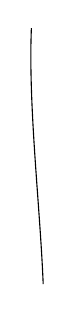
\begin{tikzpicture}[x=0.5cm,y=0.5cm]
\draw (0,6.5) .. controls (-0.08,4.5) and (0.22,2) .. (0.3,0);
\end{tikzpicture}}

(i) $\forall x\in E,\ x'\in E'$, on a
\[
x\mid\circ\mid\beta(x')\ \Longleftrightarrow\ \alpha(x)\mid\circ\mid x'
\]

(ii) $\forall A\subset E,\ A'\subset E'$, on a
\[
A\mid\circ\mid\bar\beta(A')\ \Longleftrightarrow\ \bar\alpha(A)\mid\circ\mid A'
\]

(iii) Posant, pour $\unsure{\mathscr{S}|\mathfrak{S}|\mathbb{S}}\in\deleted{\unsure{\mathscr{P}(E)}}\Sigma_E,\ \mathscr{S}'\in\Sigma_{E'}$
\[
\begin{aligned}
\alpha_{\unsure{*|\ell}}(\mathscr{S})&=\operatorname{supp}^{\circ}_{E'}(\bar\alpha(\mathscr{S}))\\
\beta_*(\mathscr{S}')&=\operatorname{supp}^{\circ}_E(\bar\beta(\mathscr{S}'))
\end{aligned}
\]
\unsure{a)} On a \deleted{\unsure{pour}} l'équivalence
\[
\deleted{\unsure{\alpha_*(A)}}\mathscr{S}\mid\circ\mid\beta_*(\mathscr{S}')\ \Longleftrightarrow\ \alpha_*(\mathscr{S})\mid\circ\mid\mathscr{S}'
\]
\inserted{b) \deleted{plus} les relations, pour $A\in\mathscr{P}(E),\ A'\in\mathscr{P}(E')$ :}
\[
\begin{aligned}
\inserted{\alpha_*(\operatorname{supp}^{\circ}_E(A))=\operatorname{supp}^{\circ}_{E'}(\bar\alpha(\unsure{A'|A}))}\\
\inserted{\beta_*(\operatorname{supp}^{\circ}_{E'}(A'))=\operatorname{supp}^{\circ}_E(\bar\beta(\unsure{B|A'})))}
\end{aligned}
\]
\deleted{De plus,}\quad\deleted{\unsure{Démonstration.}}

% margin note written sideways, slanted upwards to the right
\margin{\uline{Définition} On dit \unsure{donc|alors} \unsure{que} $\alpha$ et $\beta$ sont \inserted{\uuline{\unsure{pré}}}\unsure{transposés} l'un de l'autre.}

% The following block is crossed through by long diagonal strokes.
\deleted{\uline{\unsure{(iv)}} Ces conditions ne dépendent que des applications $\alpha_*,\beta_*$}
% Curved stroke at the left of the cancelled lower block.
\figure{\begin{tikzpicture}[x=0.5cm,y=0.5cm]
\draw (0,2.2) .. controls (-0.18,1.4) and (-0.18,0.7) .. (0.18,0);
\end{tikzpicture}}
\[
\deleted{\unsure{\alpha_*:}}
\]
\diagram{\begin{tikzcd}[ampersand replacement=\&]
\deleted{\Sigma_E}\arrow[r,shift left=0.6ex,"\deleted{\alpha_*}"] \& \deleted{\Sigma_{E'}}\arrow[l,shift left=0.6ex,"\deleted{\beta_*}"]
\end{tikzcd}}
\deleted{définies \unsure{$\beta$} par $\alpha$ et $\beta$, et en particulier ne changent pas quand on remplace $\alpha$ et $\beta$ par $\alpha',\beta'$ \unsure{définis} par}
\[
\deleted{\unsure{\alpha}\quad\alpha(x)=\operatorname{supp}^{\circ}_E\alpha(x)}
\]
% slanted
\margin{\uline{\unsure{Donc}}}

\scanpage{91}
\mspage{87}
% archive sheet number: 90

% Continuation of the block cancelled by two diagonal strokes.
\[
\begin{aligned}
\deleted{\alpha'(x)=\operatorname{supp}^{\circ}_{E'}\alpha(x)}\\
\deleted{\beta'(x)=\operatorname{supp}^{\circ}_E\beta(x).}
\end{aligned}
\]
\deleted{De plus, pour \unsure{$\alpha$} donné $\alpha$ (\inserted{ou $\alpha'$} ou $\alpha_{\unsure{*|\ell}}$ donné), il n'existe \inserted{au plus} qu'un seul $\beta_*$ qui}

\deleted{Si $\beta_1,\beta_2$ sont deux \unsure{transposés} de $\alpha$, on a $\beta'_1=\beta'_2,\ \beta_{1*}=\beta_{2*}$, et \unsure{itou} \unsure{en échangeant|en échange} \inserted{du côté} $\alpha$ si on a deux transposés $\alpha_1,\alpha_2$ de $\beta$.}

\uline{Dém} On a évidemment $(\mathrm{ii})\Rightarrow(\mathrm{i})$, en faisant $A=\{x\},\ A'=\{x'\}$, et $(\mathrm{i})\Rightarrow(\mathrm{ii})$, en notant que
\[
\begin{aligned}
A\mid\circ\mid\bar\beta(A')&\ \Longleftrightarrow\ x\mid\circ\mid\unsure{\overleftarrow\beta|\bar\beta}(x') &&\forall x\in A,\ x'\in A'\\
\unsure{\cdot}\quad\alpha(A)\mid\circ\mid A'&\ \Longleftrightarrow\ \alpha(x)\mid\circ\mid x' &&\rule{2.7cm}{0.3pt}\ .
\end{aligned}
\]

\deleted{Quand \inserted{en plus} $A,A'\in\Sigma_E$, l'équivalence \unsure{des $2$ mbrs de (ii) reste}}
Notons que les deux \unsure{mbrs|membres} de (ii) ne changent pas quand on y remplace l'un ou l'autre des termes dans la relation $\mid\circ\mid$, ou les deux, par son support. Quand $A\in\Sigma_E,A'\in\Sigma_{E'}$, cela montre que cette équivalence \deleted{signifie} équivaut à celle de (iii), donc $(\mathrm{ii})\Rightarrow(\mathrm{iii})\inserted{\text{a)}}$. \inserted{On verra b) plus bas.} \unsure{Enfin}, prouvons que $(\mathrm{iii})\Rightarrow(\mathrm{ii})$ \unsure{(p. ex.)|(p. 86)}. On écrit la relation (ii) à prouver sous la forme équivalente :

\scanpage{92}
\mspage{88}
% archive sheet number: 91

\[
\underbrace{\operatorname{supp}^{\circ}_E(A)}_{\bar A}\mid\circ\mid\operatorname{supp}^{\circ}_E(\bar\beta(A')\ \Longleftrightarrow\ \operatorname{supp}^{\circ}_{E'}(\bar\alpha(A))\mid\circ\mid\underbrace{\unsure{\operatorname{supp}^{\circ}A'}}_{\bar A'}
\tag*{(*)}
\]
\deleted{Si on \unsure{prouve} qu'on a}
\[
\deleted{\operatorname{supp}^{\circ}_E(\bar\beta(A'))=\operatorname{supp}^{\circ}_E}
\]
\deleted{\unsure{Si on pouvait}}\inserted{Or dans (iii) b)} On a supposé
\[
\left\{
\begin{aligned}
\operatorname{supp}^{\circ}_E(\bar\beta(A'))&=\operatorname{supp}^{\circ}_E(\bar\beta(\bar A'))\ \bigl(\overset{\text{\unsure{def|déf}}}=\beta_{\unsure{*|\ell}}(\bar A')\bigr)\\
\operatorname{supp}^{\circ}_{E'}(\bar\alpha(A))&=\operatorname{supp}^{\circ}_{E'}(\bar\alpha(\bar A))\ \bigl(\overset{\text{def}}=\alpha_*(\bar A)\bigr)
\end{aligned}
\right.
\tag*{(**)}
\]
on en conclut que (*) s'écrit aussi
\[
\bar A\mid\circ\mid\beta_*(\bar A')\ \Longleftrightarrow\ \alpha_*(\bar A)\mid\circ\mid\bar A'
\]
ce qui n'est autre que (iii).
\figure{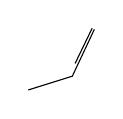
\begin{tikzpicture}[x=0.7cm,y=0.7cm]
\draw (0,0)--(0.8,0.25)--(1.2,1.1);
\draw (0.85,0.48)--(1.16,1.12);
\end{tikzpicture}}
Donc il \deleted{faut}\inserted{reste à} prouver \inserted{que (ii) \unsure{implique},} les deux relations (**) -- et il suffira \deleted{\unsure{de pr}} (par raison de symétrie) de prouver la seconde :

\uline{Corollaire 1} Sous les conditions du lemme 1 (en l'occurrence, sous la forme (ii)), si $A\in\unsure{\mathscr{P}|\mathcal{P}}(E)$, $A'\in\mathscr{P}(E')$, $\bar A=\operatorname{supp}^{\circ}_E(A)$, $\bar A'=\operatorname{supp}^{\circ}_{E'}(A')$, on a les relations (**) ci-dessus.

\uline{Dém} Comme $A\subset\bar A$, on a $\bar\alpha(A)\subset\bar\alpha(\bar A)$ d'où $\operatorname{supp}^{\circ}_{E'}(\bar\alpha(A))\subset\operatorname{supp}^{\circ}_{E'}(\bar\alpha(\bar A))$, il faut prouver $\unsure{\supset|\supseteq}$. Il revient au $=$ de dire que $\forall A'\in\Sigma_{E'}$, on a
\[
A'\mid\circ\mid\deleted{\operatorname{supp}^{\circ}_{E'}}(\bar\alpha(A))\ \Longleftrightarrow\ A'\mid\circ\mid\deleted{\unsure{\operatorname{supp}^{\circ}_{E'}}}\deleted{\unsure{\alpha_*(\bar A)}}(\bar\alpha(\bar A))
\]

\scanpage{93}
\mspage{89}
% archive sheet number: 92

% The opening argument and its implication are cancelled diagonally.
\deleted{Or par (ii), le deuxième \unsure{mbr|membre} de l'implication \unsure{à prouver} : $\beta_{\unsure{*|\ell}}(A')\mid\circ\mid A$ alors que le premier équivaut à : $A'\mid\circ\mid\bar\alpha(A)$. Donc on est ramené à voir que}
\[
\deleted{A'\mid\circ\mid\bar\alpha(A)\ \overset{?}{\Longrightarrow}\ \beta_*(A')\mid\circ\mid A}
\]

Or par (ii), les deux membres équivalent resp. à $\beta_*(A')\mid\circ\mid\unsure{A'|A}$, et $\beta_*(A')\mid\circ\mid\deleted{\unsure{\operatorname{supp}}}\bar A^{\unsure{\alpha|*}}$, où $\bar A=\operatorname{supp}A$, lesquelles sont bien équivalentes, qed.

En particulier, \deleted{\unsure{en faisant}}\inserted{faisant} $A=\{x\}$, on aura
\[
\operatorname{supp}^{\circ}_{E'}\alpha(x)=\operatorname{supp}^{\circ}_{E'}\bar\alpha(\operatorname{supp}^{\circ}_E(x))\overset{\text{\unsure{def|déf}}}=\alpha_*(\operatorname{supp}^{\circ}_E(x))
\]
i.e.
\[
\boxed{\alpha_*(\deleted{\unsure{\operatorname{supp}}}\unsure{\sigma|\varphi}_E(x))=\underbrace{\operatorname{supp}^{\circ}_{E'}(\alpha(x))}_{\alpha'(x)\ \overset{\text{def}}{\unsure{\Vert|=}}}}
\]
donc \deleted{la composée de $\alpha$ avec $\operatorname{supp}^{\circ}_{E'}$ est}

$\alpha_*$ et $\alpha'$ se déterminent mutuellement par cette formule et par la formule, évidente quelle que soit $\alpha:E\unsure{\text{---}|\longrightarrow}\unsure{\mathscr{P}|\mathcal{P}}(E')$ (permettant \inserted{$\unsure{\alpha_*|\alpha}$} de définir $\alpha'$ par composition avec $\operatorname{supp}^{\circ}_{E'}$) :
\[
\boxed{\alpha_*(S)=\underset{x\in S}{\operatorname{Sup}_{(\Sigma_{E'})}}\alpha'(x)}\quad(=\alpha'_*(S))
\]

Les conditions de Prop. 3 sur $(\alpha,\beta)$ ne dépendent que des $\alpha',\beta'$ associés, \unsure{lesquelles|lesquels} \deleted{\unsure{définissent}} donnent $\alpha'_* =\alpha_*,\ \beta'_* =\beta_*$,

\scanpage{94}
\mspage{90}
% archive sheet number: 93

\[
\left\{\begin{aligned}
\alpha' &: E\ \unsure{\text{---}|\longrightarrow}\ \Sigma_{E'}\\
\beta' &: E'\ \unsure{\longrightarrow|\text{---}}\ \Sigma_E
\end{aligned}\right.
\]
\[
\left\{\begin{aligned}
\alpha_{\unsure{*|\ell}} &: \Sigma_E\longrightarrow\Sigma_{E'}\\
\beta_* &: \Sigma_{E'}\ \unsure{\text{---}|\longrightarrow}\ \Sigma_E
\end{aligned}\right.
\]
% Vertical separator immediately to the left of the NB margin block.
\figure{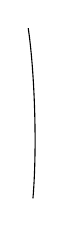
\begin{tikzpicture}[x=0.6cm,y=0.6cm]
\draw (0,0) .. controls (0.1,1.2) and (0.02,2.8) .. (-0.1,3.6);
\end{tikzpicture}}
\margin{NB. $\alpha\mapsto(\alpha'\leftrightarrow\alpha_*)$\par $\beta\mapsto(\beta'\leftrightarrow\beta_*)$}

Ceci vu, je dis que \deleted{\unsure{le}} pour $\alpha$ (ou $\alpha',\alpha_*$) donné, $\beta_*$ (ou $\beta'$) est déterminé de façon unique, par les conditions de la proposition. En effet, $\beta_*(S')$ est connu quand on connaît les $S\in\Sigma_E$ tels que $S\mid\circ\mid\beta_*(S')$, ce sont ceux pour lesquels on a $\alpha_*(S)\mid\circ\mid S'$ !

% margin note written sideways, slanted upwards to the right
\margin{\uline{\unsure{Déf}} On dit que $\alpha,\beta$ sont \inserted{\uline{pré}}transposés \unsure{l'une|l'un} de l'autre, et que $\alpha',\beta'$, ou $\alpha_*,\beta_*$ sont \uline{transposés} \unsure{l'un|l'une} de l'autre.}
% Curved separator at the lower right of the slanted margin note.
\figure{
\begin{tikzpicture}[x=0.6cm,y=0.6cm]
\draw (0,0) .. controls (-0.08,0.9) and (0.05,1.55) .. (0.55,2.05)
 -- (0.25,2.12) .. controls (0.03,2.2) and (-0.04,2.35) .. (-0.08,2.55);
\end{tikzpicture}}

Il reste à voir quelles sont les applications
\[
\alpha:E\longrightarrow\Sigma_{E'},
\]
ou ce qui revient au $=$, les applications correspondantes
\[
\alpha_*:\Sigma_E\ \unsure{\text{---}|\longrightarrow}\ \Sigma_{E'},\qquad \alpha_*(S)=\underset{x\in S}{\operatorname{Sup}_{\Sigma_{E'}}}\alpha(x)
\]
pour lesquelles il existe une $\unsure{\beta}$
\[
\beta:E'\ \unsure{\text{---}|\longrightarrow}\ \Sigma_E,
\]
\deleted{\unsure{ou ce qui revient}}\inserted{\unsure{i.e. une}}
\[
\beta_*:\Sigma_{E'}\ \unsure{\text{---}|\longrightarrow}\ \Sigma_E,\qquad \beta_*(S')=\underset{x'\in S'}{\operatorname{Sup}_{\unsure{\Sigma_E|\Sigma_{E'}}}}\beta(\unsure{x'})
\]
\unsure{transposée|transposé}.

On va quand $=$ partir de $\alpha:E\unsure{\text{---}|\longrightarrow}\unsure{\mathscr{P}|\mathcal{P}}(E')$ \unsure{ald|au lieu de} $E\unsure{\longrightarrow|\text{---}}\unsure{\Sigma|\mathscr{P}}_{E'}$.

\scanpage{95}
\mspage{91}
% archive sheet number: 94

\uline{Proposition 4} Soit $\alpha:E\ \unsure{\text{---}|\longrightarrow}\ \unsure{\mathscr{P}|\mathcal{P}}(E')$ une correspondance, \deleted{\unsure{Considérons}} posons
\[
\begin{aligned}
\alpha' &: E\longrightarrow\Sigma_{E'},\qquad \alpha'(x)\overset{\text{\unsure{def|déf}}}=\operatorname{supp}^{\circ}_{E'}(\alpha(x))\\
\alpha_{\unsure{*|\ell}} &: \Sigma_E\ \unsure{\text{---}|\longrightarrow}\ \Sigma_{E'},
\end{aligned}
\]
\[
\deleted{\unsure{\alpha_*(S)}=\underset{x\in S}{\operatorname{Sup}_{\Sigma_{E'}}}\alpha'(x)=\underset{x\in S}{\unsure{\operatorname{Sup}}}\alpha'(x)}
\]
\[
\deleted{\unsure{\operatorname{supp}^{\circ}\bar\alpha(S)}}
\]
\[
\inserted{\alpha_*(S)=\operatorname{supp}^{\circ}_{E'}(\bar\alpha(S))=\underset{x\in S}{\operatorname{Sup}_{\Sigma_{E'}}}\alpha'(x).}
\]

Conditions équivalentes :

(i) $\alpha$ admet une prétransposée
\[
\beta:E'\longrightarrow\mathscr{P}(E)
\]
ou ce qui revient au $=$, une transposée
\[
\beta':E'\ \unsure{\longrightarrow|\text{---}}\ \Sigma_E,\quad\text{ou}\quad\beta_*:\Sigma_{E'}\ \unsure{\text{---}|\longrightarrow}\ \Sigma_E.
\]

\unsure{(ii)|(v)} \inserted{a)} $\alpha_*$ commute aux $\operatorname{Sup}$ quelconques.

\inserted{b) \deleted{\unsure{$\alpha$}} $\forall x\in E$,}
\[
\inserted{\alpha_*\operatorname{supp}^{\circ}_E(x)\ \bigl(\text{i.e. }\operatorname{supp}^{\circ}_{E'}(\bar\alpha(\operatorname{supp}^{\circ}_E(x)))\bigr)=\operatorname{supp}^{\circ}_{E'}(\alpha(x))}
\]

\deleted{\unsure{(iii)}}\unsure{(ii')|(iii)} On a les formules, pour \unsure{$\forall$} $A\in\mathscr{P}(E)$
\[
\alpha_*(\overbrace{\operatorname{supp}^{\circ}_E(A)}^{\bar A})=\operatorname{supp}^{\circ}_{E'}(\bar\alpha(A))
\]
(i.e. $\bar\alpha(\bar A)$ et $\bar\alpha(A)$ ont $=$ support dans $E'$)

\unsure{(iii)|(iv)} $\forall S'\in\Sigma_{E'}$, l'ens
\[
S=\{x\in E\mid\alpha'(x)\subset S'\}
\]
dans $E$ est dans $\Sigma_E$

(iv) $\forall x'\in E'$, l'ens
\[
\deleted{\unsure{\beta|\rho}}\inserted{\unsure{\gamma|\beta}}(x')=\{x\in E\mid\alpha(x)\mid\circ\mid x'\}
\]
est dans $\Sigma_E$.
% A long curved continuation arrow runs from condition (ii) to the foot of the page.

\figure{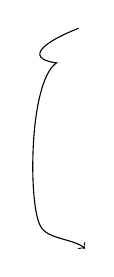
\begin{tikzpicture}[x=0.4cm,y=0.4cm]
\draw[->] (0.8,7) .. controls (-0.7,6.4) and (-0.7,6) .. (0.1,5.9) .. controls (-0.8,5.3) and (-0.8,1.3) .. (-0.4,0.7) .. controls (-0.2,0.3) and (0.7,0.3) .. (1,0);
\end{tikzpicture}}

\scanpage{96}
\mspage{92}
% archive sheet number: 95

\uline{Dém} Prouvons d'abord
\[
(\mathrm{i})\Rightarrow\unsure{(\mathrm{ii}')|(\mathrm{iii})}\Rightarrow(\mathrm{iii})\Rightarrow(\mathrm{iv})\Rightarrow(\mathrm{i}),
\]
ce qui établira l'équivalence de \unsure{ttes|toutes} les conditions sauf \unsure{(ii)|(v)}

$(\mathrm{i})\Rightarrow(\mathrm{ii}')$ a été vu

$(\mathrm{ii}')\Rightarrow(\mathrm{iii})$. \deleted{Soit $\unsure{T'|S'}=\unsure{C|\complement}S'$. On a alors, pour}
Soit $\bar S=\operatorname{supp}^{\circ}_E S\supset S$ On a
\deleted{$x\in E$}\quad\deleted{$S\subset\bar S$, \unsure{déf et}}
\[
\deleted{x\in S\Longleftrightarrow\alpha(x)\subset S'\Longleftrightarrow\alpha(x)\unsure{\mid}}
\]
par (ii'), $\bar\alpha(S)$ et $\bar\alpha(\bar S)$ ont $=$ support dans $E'$, \deleted{\unsure{et}} comme $S'$ est un support, $\bar\alpha(S)\subset S'\Rightarrow\bar\alpha(\bar S)\subset S'$, donc $\bar S\subset S$ par définition de $S$, donc $S=\bar S$, i.e. $S\in\Sigma_E$.

$(\mathrm{iii})\Rightarrow(\mathrm{iv})$ tautologique, prenant $S'=\operatorname{cosupp}^{\circ}\{x'\}$.

$(\mathrm{iv})\Rightarrow(\mathrm{i})$, on trouve la transposée
\[
\beta(x')=C\gamma(x')\quad\unsure{.|\ldots}
\]
En effet, \deleted{la relation}\inserted{je dis} qu'on a, pour $x\in E,x'\in E'$
\[
x\mid\circ\mid\beta(x')\ \Longleftrightarrow\ \alpha(x)\mid\circ\mid x'
\]
\deleted{\unsure{i.e. $x$}}\inserted{\unsure{i.e.}} i.e.
\[
\deleted{\unsure{\operatorname{supp}^{\circ}_E(x)\subset}}
\]
\[
x\in C\beta(x')=\gamma(x')
\]
ce qui n'est autre que la définition de $\gamma(x')$.

Je dis que les conditions \inserted{équiv. (i) à (iv)} impliquent \unsure{(ii)|(v)}. En effet, \deleted{\unsure{comme}}\inserted{b) est clair par (ii') et pour a)} Soit $(S_i)_{i\in I}$, $S_i\in\Sigma_E$, $S=\operatorname{Sup}^{\deleted{\unsure{\Sigma}}}_{\Sigma_E}S_i=\operatorname{supp}^{\circ}_E(\bigcup S_i)$. On aura \unsure{donc}
\[
\alpha_{\unsure{*|\ell}}(S)=\alpha_*(\operatorname{supp}^{\circ}_E(\bigcup S_i))=\operatorname{supp}^{\circ}_{E'}(\underbrace{\bar\alpha(\bigcup S_i)}_{\bigcup_i\bar\alpha(S_i)})
\]

\scanpage{97}
\mspage{93}
% archive sheet number: 96

\[
=\operatorname{supp}^{\circ}_{E'}\bigcup_i\underbrace{\operatorname{supp}^{\circ}_{E'}(\bar\alpha(S_i))}_{\alpha_{\unsure{*|\ell}}(S_i)}=\underset{i}{\operatorname{Sup}}\alpha_*(S_i),\quad\text{\unsure{qed.|QED.}}
\]

Il reste à prouver que (v) implique le reste. \unsure{p. ex.} sous la forme \unsure{(ii') ?|(ii')}
\[
\alpha_*(\operatorname{supp}^{\circ}_E(A))\overset{?}{=}\operatorname{supp}^{\circ}_{E'}(\bar\alpha(A))
\]
Or on a
\[
\operatorname{supp}^{\circ}_E(A)=\underset{\unsure{x'|x}\in A}{\operatorname{Sup}_{\Sigma_E}}\sigma_E(x)
\]
d'où, par (v)
\[
\alpha_*(\operatorname{supp}^{\circ}_E(A))=\underset{x\in A}{\operatorname{Sup}_{\Sigma_{E'}}}\alpha_*(\sigma_E(x))
\]
et d'autre part
\[
\operatorname{supp}^{\circ}_{E'}(\underbrace{\bar\alpha(A)}_{\bigcup_{x\in A}\alpha(x)})=\underset{x\in A}{\operatorname{Sup}_{\Sigma_{E'}}}{\unsure{\operatorname{supp}|\operatorname{Supp}}}^{\circ}_{E'}\alpha(x)
\]
et on gagne, pourvu que l'on \unsure{sache}
\[
\alpha_*(\deleted{\unsure{\sigma_E(x)}}\operatorname{supp}^{\circ}_E(x))=\operatorname{supp}^{\circ}_{E'}(\alpha(x))
\]
c'est v b), que j'ai dû rajouter après-coup.

\deleted{La condition v b) signifie aussi que}

\uline{Cor.} \deleted{Soit}\inserted{Soient} $\Sigma=\Sigma_{\underline E},\ \Sigma'=\Sigma_{\underline{E'}}$, soit
\[
\operatorname{Corr}(\Sigma,\Sigma')
\]
l'ens des applications
\[
\alpha_*:\Sigma\longrightarrow\Sigma'
\]
qui commutent aux $\operatorname{Sup}$ quelconques (appelons les ``correspondances'' \deleted{\unsure{de}} de $\Sigma$ \unsure{à|:} $\Sigma'$) (elles sont donc croissantes), et
\[
\operatorname{Corr}(\underline E,\underline{E'})\qquad\deleted{\unsure{k|\alpha}}
\]
